\section{Citus}
\label{sec:citus}

\href{https://www.citusdata.com/}{Citus}~--- горизонтально масштабируемый PostgreSQL кластер. Citus использует механизм расширений PostgreSQL вместо того, что бы использовать модифицированную версию базы (как это делает <<\ref{sec:postgres-xc}~\nameref{sec:postgres-xc}>> или <<\ref{sec:postgres-xl}~\nameref{sec:postgres-xl}>>), что позволяет использовать новые версии PostgreSQL с новыми возможностями, сохраняя при этом совместимость с существующими PostgreSQL инструментами. Кластер предоставляет пользователям результаты запросов в режиме <<реального времени>> для большого и растущего обьема данных (благодаря параллелизации запросов между нодами). Примеры использования:

\begin{itemize}
  \item аналитика и вывод данных в реальном времени на графики;
  \item хранение большого набора данных для архива и создание отчетов по ним;
  \item анализ и сегментация большого обьема данных;
\end{itemize}

Нагрузки, которые требуют большой поток данных между узлами кластера, как правило, не будет хорошо работать с Citus кластером. Например:

\begin{itemize}
  \item традиционные хранилища данных с длительными и в свободном формате SQL запросами (data warehousing);
  \item множественные распределенные транзакции между несколькими шардами;
  \item запросы, которые возвращают данные по тяжелым \href{https://ru.wikipedia.org/wiki/ETL}{ETL} запросам;
\end{itemize}



\subsection{Архитектура}

На верхнем уровне Citus кластер распределяет данные по PostgreSQL экземплярам. Входящие SQL запросы затем обрабатываются паралельно через эти сервера.

\begin{figure}[ht!]
  \center{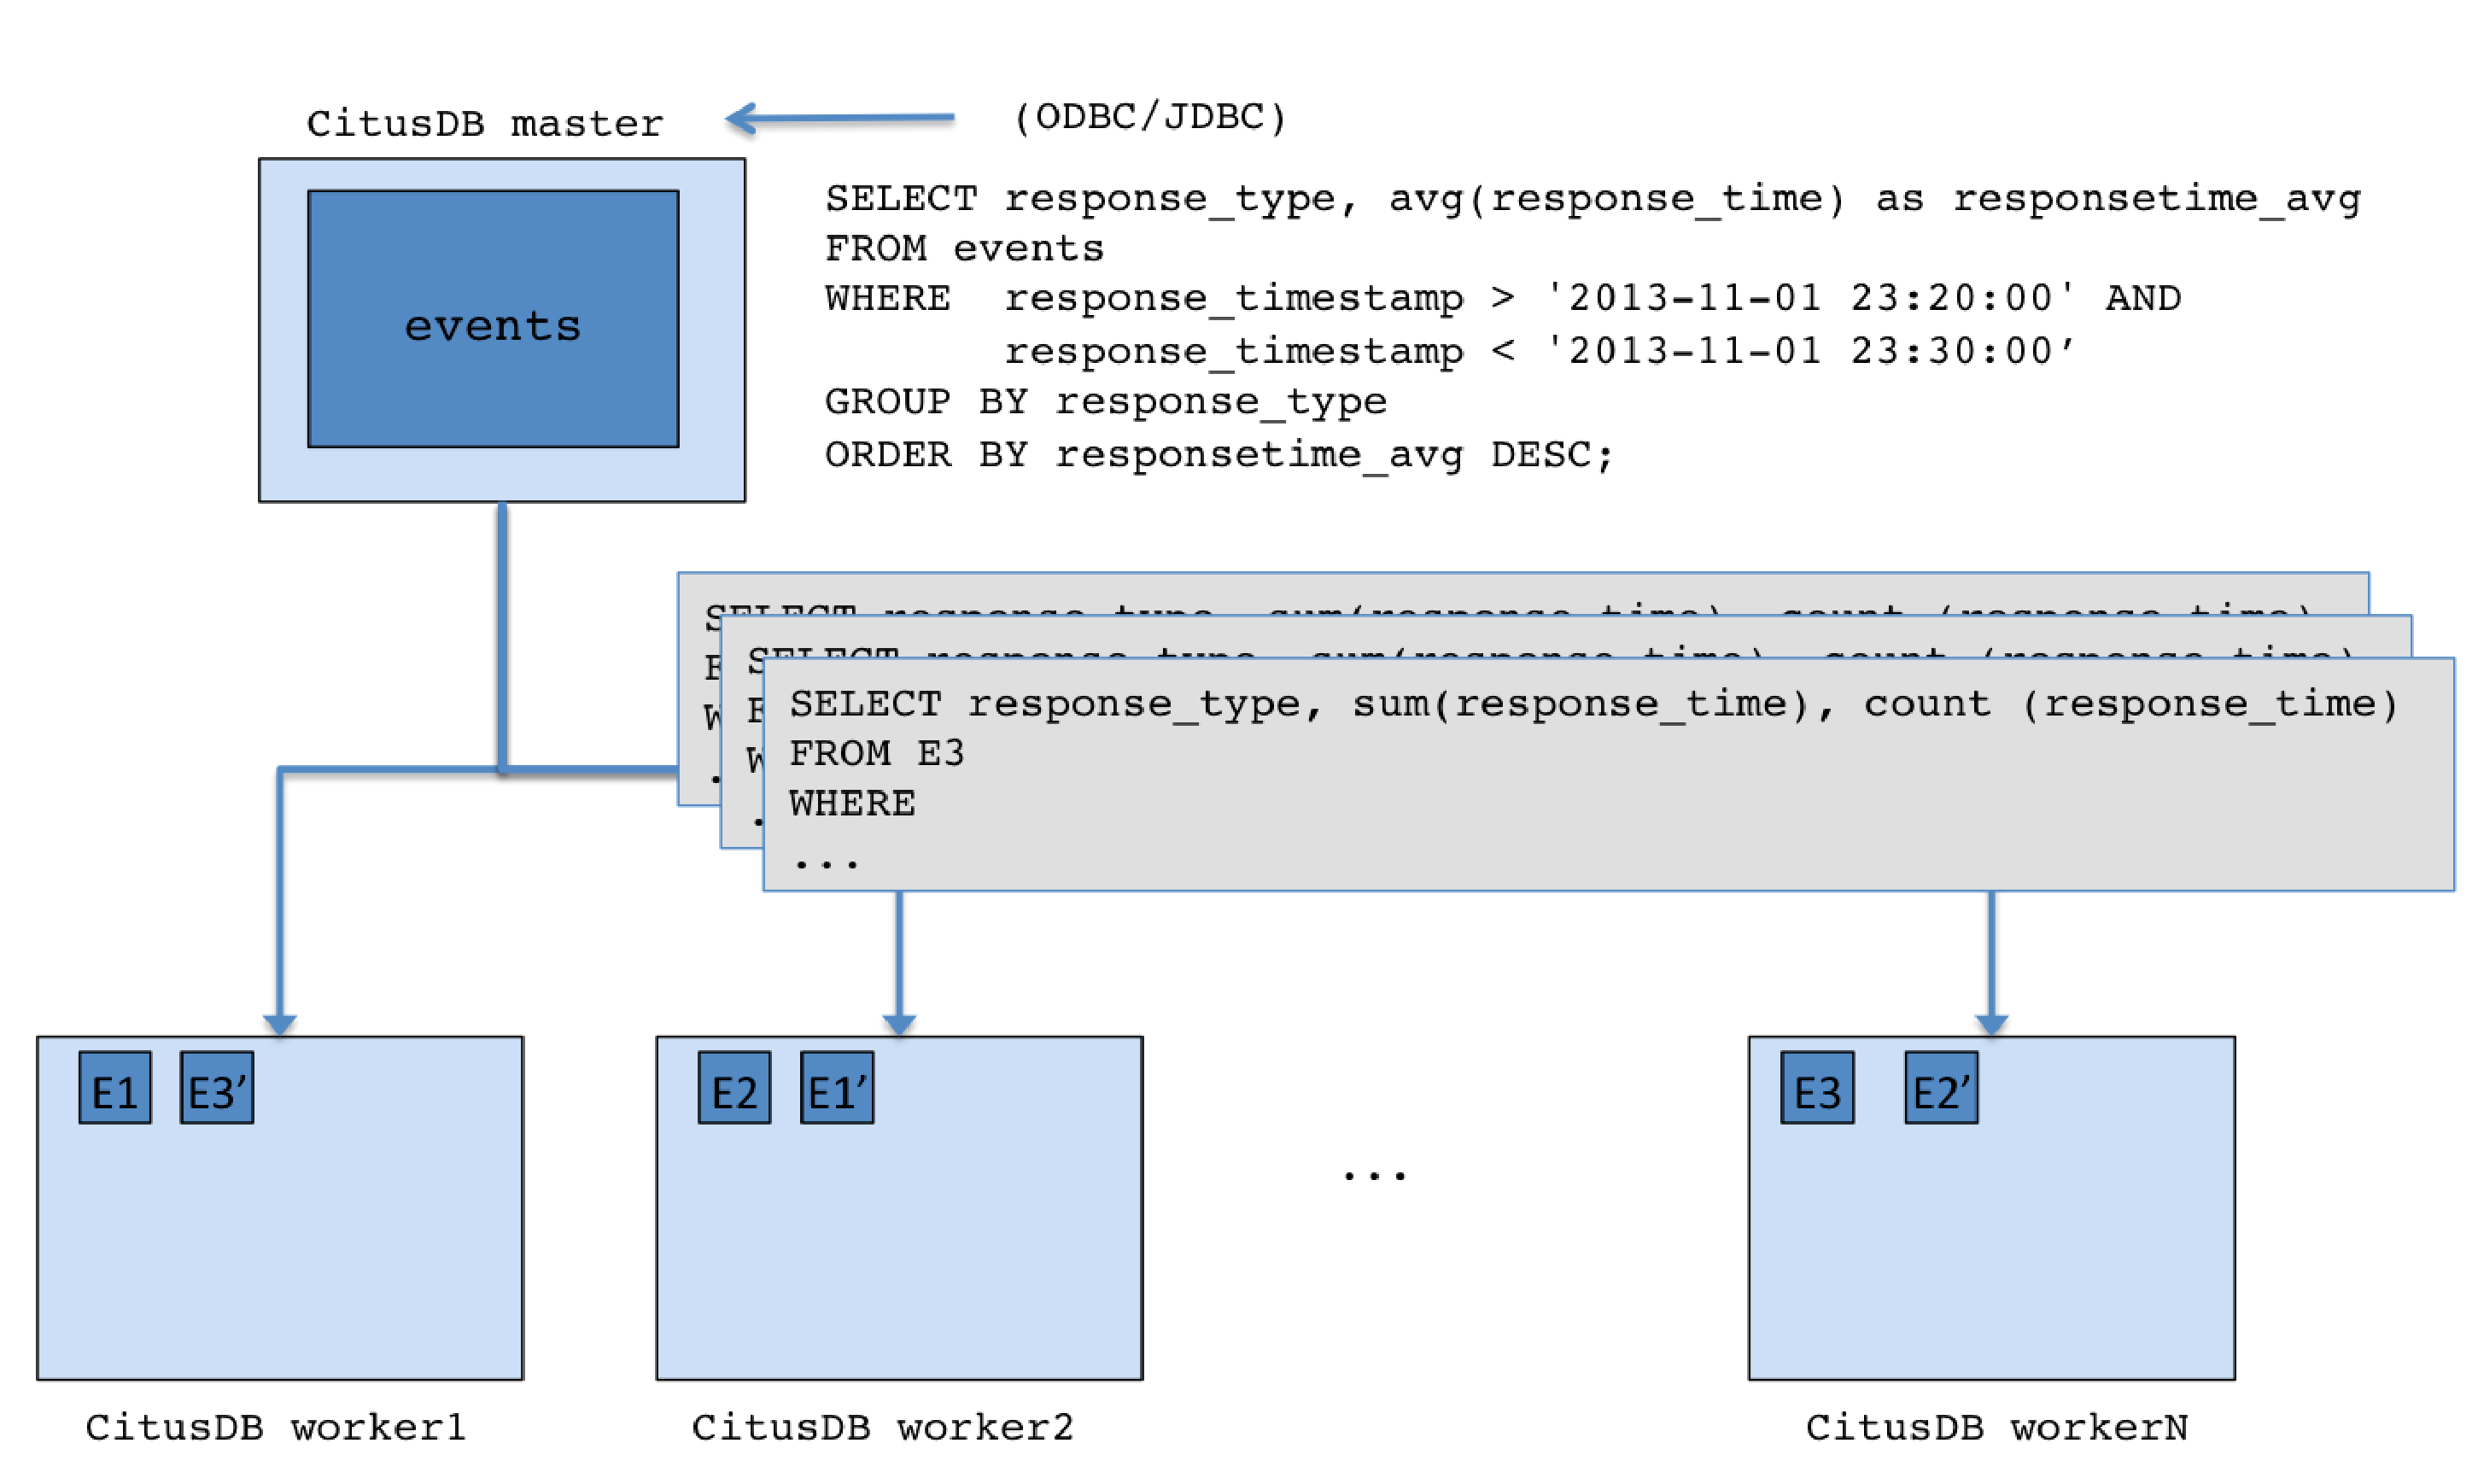
\includegraphics[width=1\textwidth]{citus-basic-arch.pdf}}
  \caption{Архитектура Citus кластера}
  \label{fig:citus_basic_arch}
\end{figure}

При разворачивании кластера один из экземпляров PostgreSQL выбирается в качестве мастер (master) ноды. Затем остальные добавляются как PostgreSQL воркеры (worker) в конфигурационном файле мастер ноды. После этого все взаимодействие с кластером ведется через мастер ноду с помощью стандартных PostgreSQL интерфейсов. Все данные распределены по воркерам. Мастер хранит только  метаданные о воркерах.

Citus использует модульную архитектуру для блоков данных, которая похожа на \href{https://ru.wikipedia.org/wiki/Hadoop#HDFS}{HDFS} (Hadoop Distributed File System), но использует PostgreSQL таблицы вместо файлов. Каждая из этих таблиц представляет собой горизонтальный раздел или логический <<шард>> (shard). Каждый шард дублируется, по крайней мере, на двух воркерах (можно настроить это на более высокое значение). В результате, потеря одной машины не влияет на доступность данных. Логическая архитектура шардинга в Citus также позволяет добавлять новые воркеры, чтобы увеличить пропускную способность и вычислительную мощность кластера.

Citus мастер содержит таблицы метаданных для отслеживания всех воркеров и расположение шардов базы данных на них. Эти таблицы также ведут статистику, такую как размер и минимальное/максимальное значений в шардах, которые помогают распределеннию SQL запросов Citus планировщику. Таблицы метаданных небольшие (обычно несколько мегабайт), и могут быть дублированы и быстро восстановлены, если с мастером когда-либо произойдет сбой. Подробнее про таблицах метаданных можно глянуть \href{https://docs.citusdata.com/en/v5.1/reference/metadata_tables.html}{в документации}.

Когда кластер получает SQL запрос, Citus мастер делит его на более мелкие фрагменты запросов, где каждый фрагмент может выполняться независимо на воркере. Это позволяет Citus распределять каждый запрос в кластере, используя вычислительные мощности всех задействованных узлов, а также отдельных ядер на каждом узле. Мастер затем поручает воркерам выполнить запрос, осуществляет контроль за их исполнением, объединяет результаты по запросам и возвращает конечный результат пользователю. Для того, чтобы гарантировать, что все запросы выполняются в масштабируемой манере, мастер также применяет оптимизации, которые сводят к минимуму объем данных, передаваемых по сети.

Citus кластер может легко переносить сбои воркеров из-за своей логической шардинг архитектуре. Если воркер терпит неудачу во время выполнения запроса, Citus завершает запрос, направляя неудачные части запроса другим воркерам, которые имеют копию данных. Если воркер находится в не рабочем состоянии (сервер упал), пользователь может легко произвести ребалансировку кластера, чтобы поддерживать тот же уровень доступности.


\subsection{Установка}

Установка Citus кластера не требует особых усилий. Для использовании в боевом окружении лучше изучить \href{https://docs.citusdata.com/en/v5.1/installation/production.html}{данную документиацию}. Для проверки, что кластер работает и мастер видит воркеры можно выполнить команду \lstinline!master_get_active_worker_nodes!, которая покажет список воркеров:

\begin{lstlisting}[language=SQL,label=lst:citus1,caption=Список воркеров]
postgres=# select * from master_get_active_worker_nodes();
 node_name | node_port
-----------+-----------
 localhost |      9702
 localhost |      9701
(2 rows)
\end{lstlisting}


\subsection{Распределенные таблицы}

